
\let\negmedspace\undefined
\let\negthickspace\undefined
\documentclass[journal]{IEEEtran}
\usepackage[a5paper, margin=10mm, onecolumn]{geometry}
%\usepackage{lmodern} % Ensure lmodern is loaded for pdflatex
\usepackage{tfrupee} % Include tfrupee package
\setlength{\headheight}{1cm} % Set the height of the header box
\setlength{\headsep}{0mm}     % Set the distance between the header box and the top of the text
\usepackage{gvv-book}
\usepackage{gvv}
\usepackage{cite}
\usepackage{amsmath,amssymb,amsfonts,amsthm}
\usepackage{algorithmic}
\usepackage{graphicx}
\usepackage{textcomp}
\usepackage{xcolor}
\usepackage{txfonts}
\usepackage{listings}
\usepackage{enumitem}
\usepackage{mathtools}
\usepackage{gensymb}
\usepackage{comment}
\usepackage[breaklinks=true]{hyperref}
\usepackage{tkz-euclide} 
\usepackage{listings}
% \usepackage{gvv}                                        
\def\inputGnumericTable{}                                 
\usepackage[latin1]{inputenc}                                
\usepackage{color}                                            
\usepackage{array}                                            
\usepackage{longtable}                                       
\usepackage{calc}                                             
\usepackage{multirow}                                         
\usepackage{hhline}                                           
\usepackage{ifthen}                                           
\usepackage{lscape}
\renewcommand{\thefigure}{\theenumi}
\renewcommand{\thetable}{\theenumi}
\setlength{\intextsep}{10pt} % Space between text and floats
\numberwithin{equation}{enumi}
\numberwithin{figure}{enumi}
\renewcommand{\thetable}{\theenumi}
\begin{document}
\bibliographystyle{IEEEtran}
\title{10.4.2.1.3}
\author{EE24BTECH11041 - Mohit}
% \maketitle
% \newpage
% \bigskip
{\let\newpage\relax\maketitle}
\begin{enumerate}
\item Find the roots of the following quadratic equations by factorisation.
\begin{align}
\sqrt{2}x^2 + 7x + 5\sqrt{2} = 0
\end{align}
\textbf{Theoritical Solution-}\\
Checking roots of equation exist or not,

\begin{align}
b^2 - 4ac \geq 0 \\
= 49 - 4(\sqrt{2})\brak{5\sqrt{2}}\\
= 9 
\end{align}
This means roots of equation exist.\\
And its roots are given by 
\begin{align}
x = \frac{b-\sqrt{b^2-4ac}}{2a},\frac{b+\sqrt{b^2-4ac}}{2a}\\
x = -\sqrt{2},-\frac{5}{\sqrt{2}}
\end{align}
\textbf{CODING LOGIC:-}


\textbf{Newton-Raphson Method}
\begin{enumerate}
\item Update Equation:
\begin{align}
 x_{n+1} = x_n - \frac{f(x_n)}{f'(x_n)}   
\end{align}

\item Steps:\\
1. Start with an initial guess $ x_0 $.\\
2. Define the function \( f(x) \) and its derivative  $f'(x)$.\\
3. Iterate using:
   \begin{align}
   x_{n+1} = x_n - \frac{f(x_n)}{f'(x_n)}
   \end{align}
   until convergence, i.e.,
   \begin{align}
   \abs{x_{n+1} - x_n} < \text{tolerance}
   \end{align}
4. Stop if $f'(x_n)$ is close to zero to avoid division by zero.

\item Convergence Criteria:
The method converges quadratically if the initial guess is sufficiently close to the root and  $f'(x) \neq 0 $.
\end{enumerate}

\textbf{Secant Method}
\begin{enumerate}
\item{Update Formula:}
\begin{align}
x_{n+1} = x_n - f(x_n) \cdot \frac{x_n - x_{n-1}}{f(x_n) - f(x_{n-1})}    
\end{align}


\item{Steps:}\\
1. Start with two initial guesses $x_0$  and $x_1$.\\
2. Define the function $f(x)$.\\
3. Iterate using:
   \begin{align}
   x_{n+1} = x_n - f(x_n) \cdot \frac{x_n - x_{n-1}}{f(x_n) - f(x_{n-1})}    
   \end{align}
   until convergence, i.e.,
   \begin{align}
   \abs{x_{n+1} - x_n} < \text{tolerance}.
   \end{align}
4. Stop if $ f(x_n) - f(x_{n-1}) $ is close to zero to avoid division by zero.

\item{Convergence Criteria:}
The method converges superlinearly and does not require the derivative $ f'(x) $.


\end{enumerate}

\begin{figure}[h!]
   \centering
   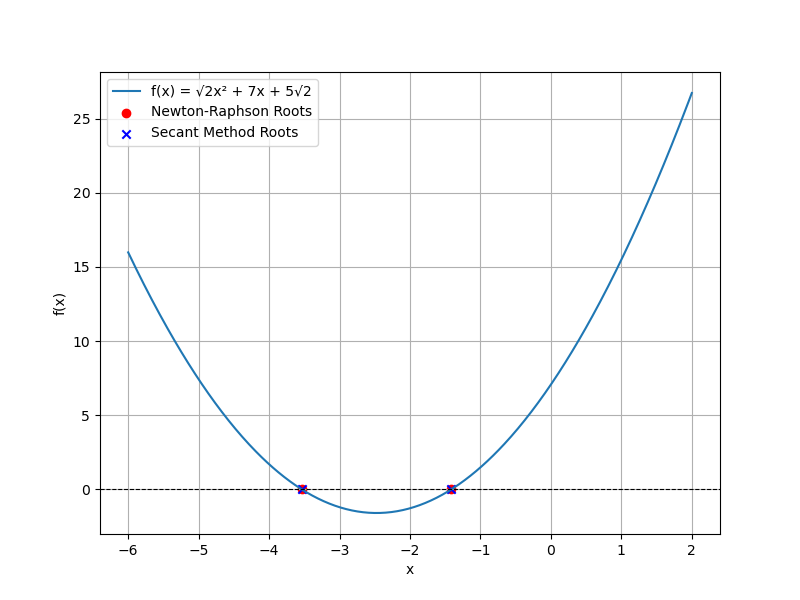
\includegraphics[width=0.7\linewidth]{figs/Figure_1.png}
\end{figure}


\textbf{CODING LOGIC FOR FINDING EIGENVALUES :-}\\


The quadratic equation 
\begin{align}
\sqrt{2}x^2 + 7x + 5\sqrt{2} = 0
\end{align}
is rewritten in matrix form:
\begin{align}
\text{Matrix} =
\myvec{0 & -\frac{c}{a} \\
1 & -\frac{b}{a}
}
\end{align}

\begin{align}
a = \sqrt{2}, \quad b = 7, \quad c = 5\sqrt{2}.
\end{align}

Substituting the values of $a,b$ and $c$, the matrix becomes:\\
Let
\begin{align}
\text{A} =
\myvec{0 & -5 \\
1 & -\frac{7}{\sqrt{2}}
}
\end{align}
\textbf{QR-DECOMPOSITION:-GRAM-SCHMIDT METHOD}\\



\begin{enumerate}

\item QR decomposition 
\begin{align}
A = QR
\end{align}
\begin{enumerate}
    \item $Q$ is an $ m \times n $ orthogonal matrix
    \item $R$ is an $n \times n$ upper triangular matrix.
\end{enumerate}
Given a matrix $ A = [a_1, a_2, \dots, a_n] $, where each $ a_i $ is a column vector of size $ m \times 1 $.

\item Normalize the first column of $A$:
\begin{align}
q_1 = \frac{a_1}{\norm{a_1}}
\end{align}

\item  For each subsequent column $ a_i $, subtract the projections of the previously obtained orthonormal vectors from $ a_i $ :
\begin{align}
a_i' = a_i - \sum_{k=1}^{i-1} \langle a_i, q_k \rangle q_k
\end{align}
Normalize the result to obtain the next column of \( Q \):
\begin{align}
q_i = \frac{a_i'}{\norm{a_i'}}
\end{align}

Repeat this process for all columns of \( A \).

\item Finding $R$:- \\
After constructing the ortho-normal columns $ q_1, q_2, \dots, q_n $ of $Q$, we can compute the elements of $R$ by taking the dot product of the original columns of $A$ with the columns of $Q$:

\begin{align}
    r_{ij} = \langle a_j, q_i \rangle \text{ , for  }  i \leq j 
\end{align}
\end{enumerate}



\textbf{QR-Algorithm}\\
\begin{enumerate}
\item Initialization \\
Let $A_0 = A $, where $A$ is the given matrix.

\item QR Decomposition \\
For each iteration $ k = 0, 1, 2, \dots $:
\begin{enumerate}
    \item Compute the QR decomposition of \( A_k \), such that:
    \begin{align}
    A_k = Q_k R_k
    \end{align}
    where:
    \begin{enumerate}
        \item $Q_k $ is an orthogonal matrix ($ Q_k^\top Q_k = I $).
        \item $ R_k $ is an upper triangular matrix.
    \end{enumerate}
    The decomposition ensures $ A_k = Q_k R_k $.

    \item Form the next matrix \( A_{k+1} \) as:
    \begin{align}
    A_{k+1} = R_k Q_k
    \end{align}
\end{enumerate}

\item Convergence\\
Repeat Step 2 until $ A_k $ converges to an upper triangular matrix $ T $. The diagonal entries of $T$ are the eigenvalues of $A$.\\
\item The eigenvalues of matrix will be the roots of the equation.


\end{enumerate}


\begin{figure}[h!]
   \centering
   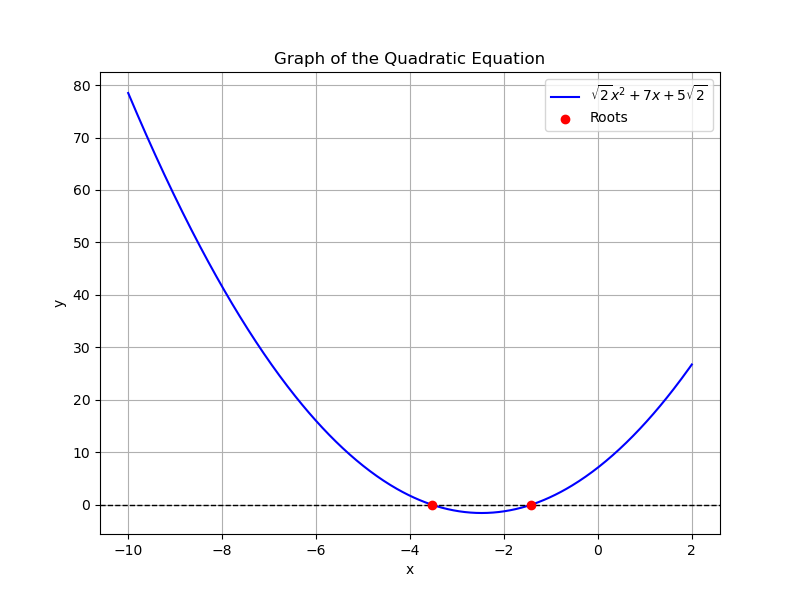
\includegraphics[width=0.7\linewidth]{figs/Figure_2.png}
\end{figure}
\end{enumerate}
\end{document}
